\documentclass[PLAIN]{Lilly}
\begin{document}
\pagenumbering{arabic}
\tableofcontents \clearpage 
\begin{lstplain}[language=lLatex]
%%Einbindung erfolgt über:
\getGraphics{:lan:Pfad:ran:}
 \end{lstplain}
\begin{tabularx}{\linewidth}{^m{0.5\linewidth}^>{\centering\arraybackslash}m{0.5\linewidth}+}
\toprule\headerrow Pfad & Ergebnis\\
\midrule

\phantomsection \addcontentsline{toc}{chapter}{Allerlei}
\phantomsection \addcontentsline{toc}{section}{Teufel}\verb|Allerlei/Teufel|\quad{\tiny pdf}& 
\includegraphics[width=0.8\linewidth]{Allerlei/Teufel-pdf.pdf}\\
\midrule 
\phantomsection \addcontentsline{toc}{chapter}{Automat}
\phantomsection \addcontentsline{toc}{section}{AutomatDFA}\verb|Automat/AutomatDFA|\quad{\tiny pdf}& 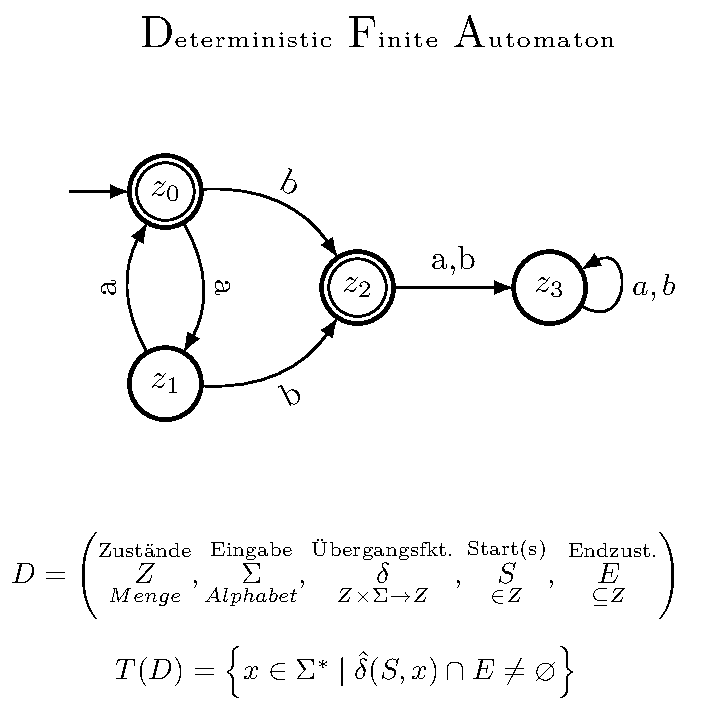
\includegraphics[width=0.8\linewidth]{Automat/AutomatDFA-pdf.pdf}\\
\midrule \phantomsection \addcontentsline{toc}{section}{AutomatNFA}\verb|Automat/AutomatNFA|\quad{\tiny pdf}& 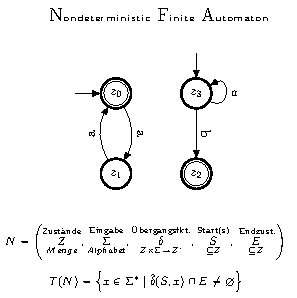
\includegraphics[width=0.8\linewidth]{Automat/AutomatNFA-pdf.pdf}\\
\midrule \phantomsection \addcontentsline{toc}{section}{CYKAlgorithmus}\verb|Automat/CYKAlgorithmus|\quad{\tiny pdf}& 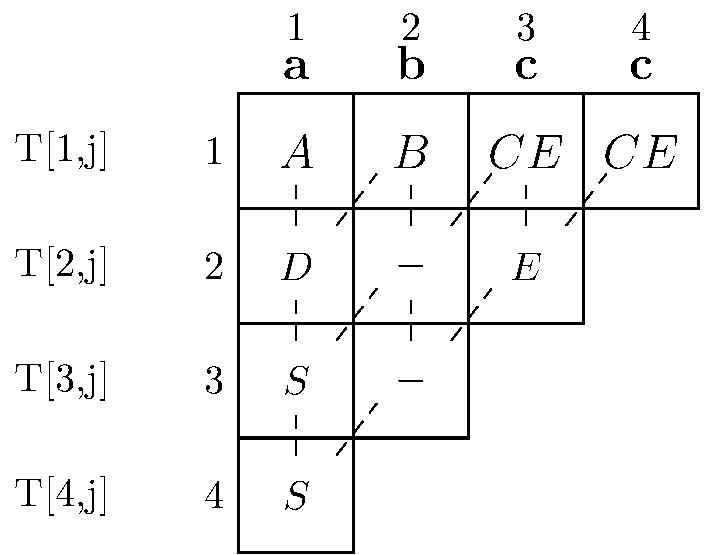
\includegraphics[width=0.8\linewidth]{Automat/CYKAlgorithmus-pdf.pdf}\\
\midrule \phantomsection \addcontentsline{toc}{section}{Demo-1}\verb|Automat/Demo-1|\quad{\tiny pdf}& 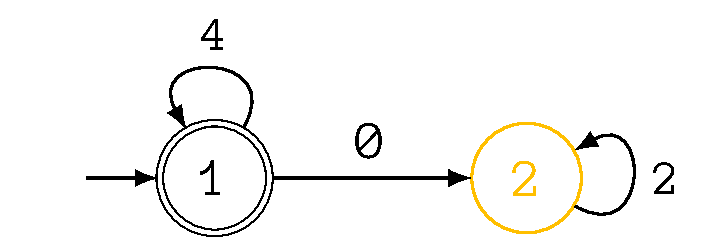
\includegraphics[width=0.8\linewidth]{Automat/Demo-1-pdf.pdf}\\
\midrule \phantomsection \addcontentsline{toc}{section}{Demo-2}\verb|Automat/Demo-2|\quad{\tiny pdf}& 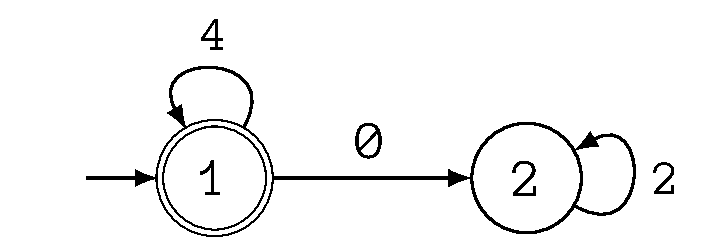
\includegraphics[width=0.8\linewidth]{Automat/Demo-2-pdf.pdf}\\
\midrule \phantomsection \addcontentsline{toc}{section}{Demo}\verb|Automat/Demo|\quad{\tiny pdf}& 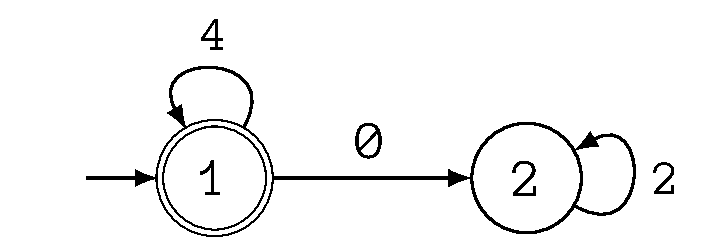
\includegraphics[width=0.8\linewidth]{Automat/Demo-pdf.pdf}\\
\midrule \phantomsection \addcontentsline{toc}{section}{Header}\verb|Automat/Header|\quad{\tiny pdf}& 
\includegraphics[width=0.8\linewidth]{Automat/Header-pdf.pdf}\\
\midrule \phantomsection \addcontentsline{toc}{section}{MealyAutomat}\verb|Automat/MealyAutomat|\quad{\tiny pdf}& 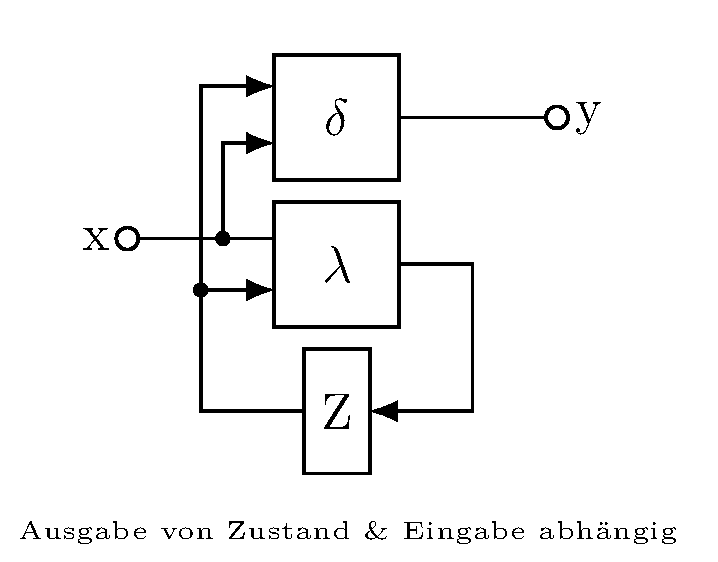
\includegraphics[width=0.8\linewidth]{Automat/MealyAutomat-pdf.pdf}\\
\midrule \phantomsection \addcontentsline{toc}{section}{MinimalautomatBeispiel/MinimalautomatBeispiel1}\verb|Automat/MinimalautomatBeispiel/MinimalautomatBeispiel1|\quad{\tiny pdf}& 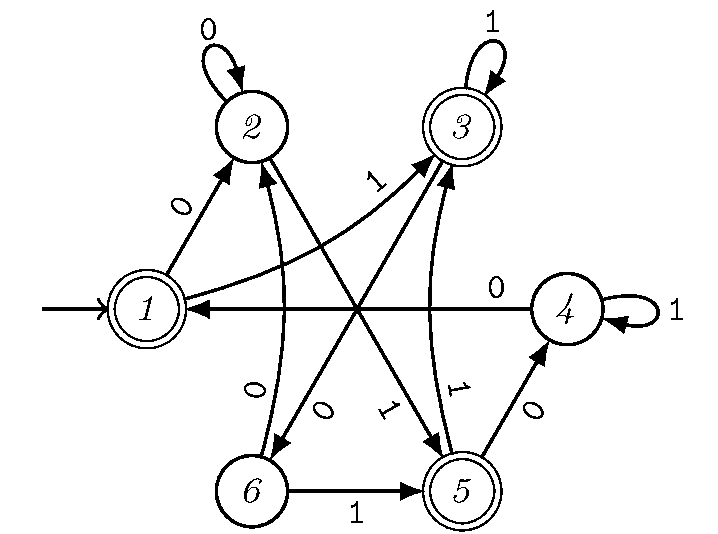
\includegraphics[width=0.8\linewidth]{Automat/MinimalautomatBeispiel/MinimalautomatBeispiel1-pdf.pdf}\\
\midrule \phantomsection \addcontentsline{toc}{section}{MinimalautomatBeispiel/MinimalautomatBeispiel2}\verb|Automat/MinimalautomatBeispiel/MinimalautomatBeispiel2|\quad{\tiny pdf}& 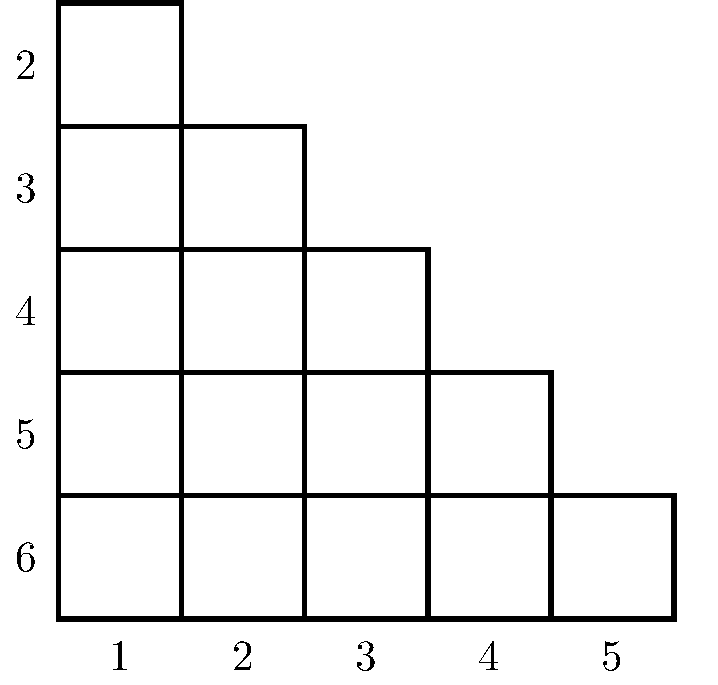
\includegraphics[width=0.8\linewidth]{Automat/MinimalautomatBeispiel/MinimalautomatBeispiel2-pdf.pdf}\\
\midrule \phantomsection \addcontentsline{toc}{section}{MinimalautomatBeispiel/MinimalautomatBeispiel3}\verb|Automat/MinimalautomatBeispiel/MinimalautomatBeispiel3|\quad{\tiny pdf}& 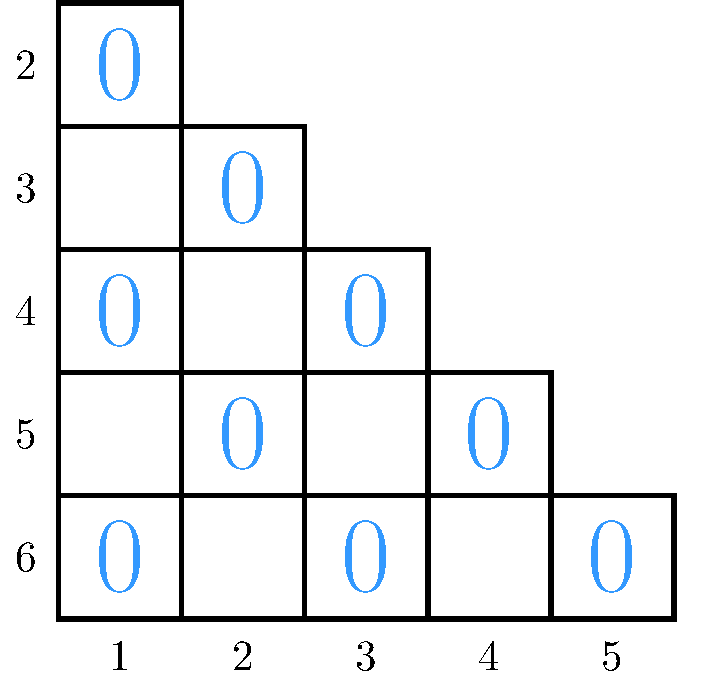
\includegraphics[width=0.8\linewidth]{Automat/MinimalautomatBeispiel/MinimalautomatBeispiel3-pdf.pdf}\\
\midrule \phantomsection \addcontentsline{toc}{section}{MinimalautomatBeispiel/MinimalautomatBeispiel4}\verb|Automat/MinimalautomatBeispiel/MinimalautomatBeispiel4|\quad{\tiny pdf}& 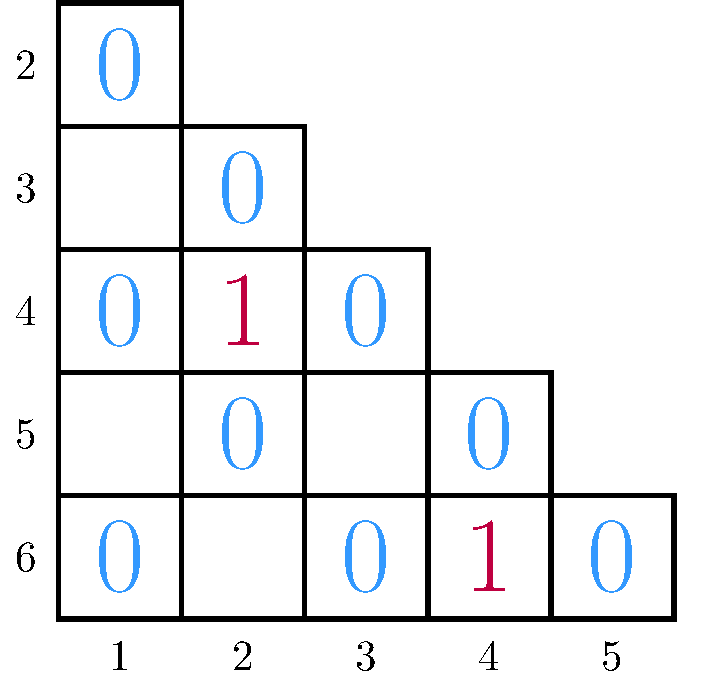
\includegraphics[width=0.8\linewidth]{Automat/MinimalautomatBeispiel/MinimalautomatBeispiel4-pdf.pdf}\\
\midrule \phantomsection \addcontentsline{toc}{section}{MinimalautomatBeispiel/MinimalautomatBeispiel5}\verb|Automat/MinimalautomatBeispiel/MinimalautomatBeispiel5|\quad{\tiny pdf}& 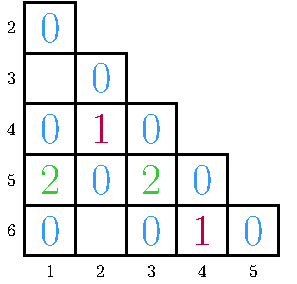
\includegraphics[width=0.8\linewidth]{Automat/MinimalautomatBeispiel/MinimalautomatBeispiel5-pdf.pdf}\\
\midrule \phantomsection \addcontentsline{toc}{section}{MinimalautomatBeispiel/MinimalautomatBeispiel6}\verb|Automat/MinimalautomatBeispiel/MinimalautomatBeispiel6|\quad{\tiny pdf}& 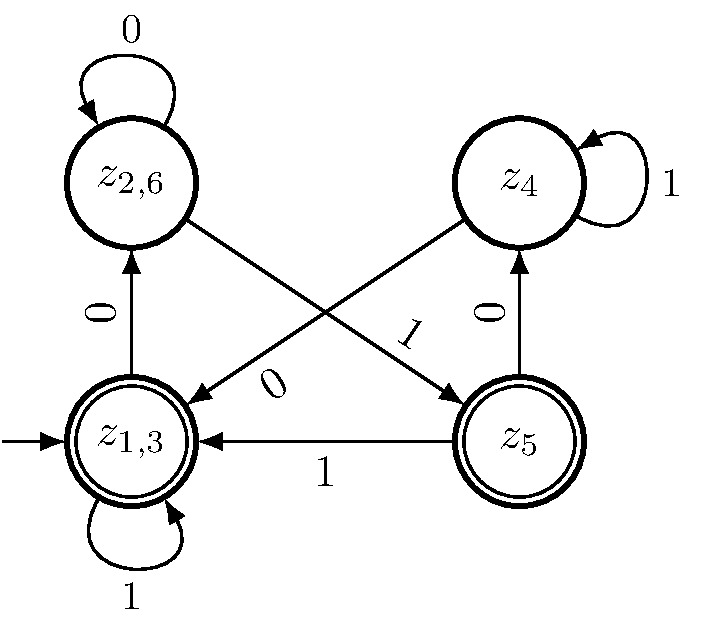
\includegraphics[width=0.8\linewidth]{Automat/MinimalautomatBeispiel/MinimalautomatBeispiel6-pdf.pdf}\\
\midrule \phantomsection \addcontentsline{toc}{section}{MooreAutomat}\verb|Automat/MooreAutomat|\quad{\tiny pdf}& 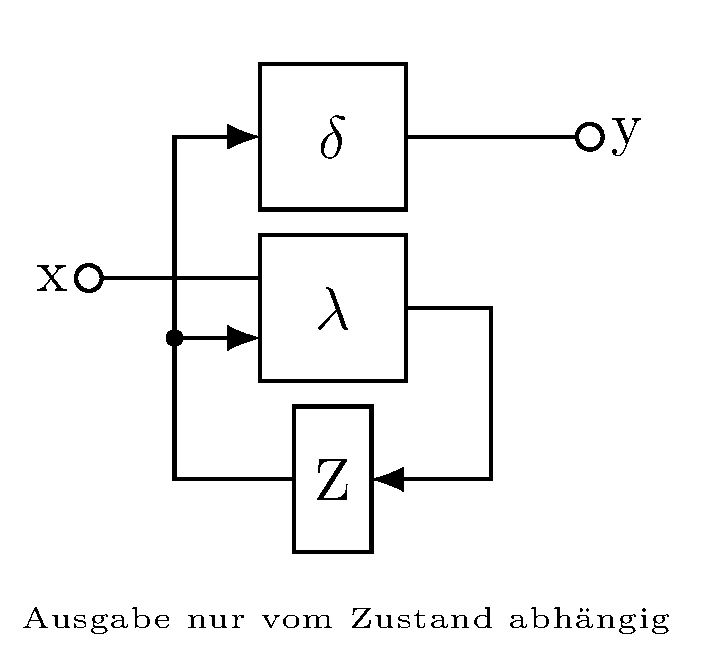
\includegraphics[width=0.8\linewidth]{Automat/MooreAutomat-pdf.pdf}\\
\midrule 
\phantomsection \addcontentsline{toc}{chapter}{Datenbanken}
\phantomsection \addcontentsline{toc}{section}{ERMExample}\verb|Datenbanken/ERMExample|\quad{\tiny pdf}& 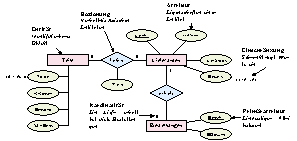
\includegraphics[width=0.8\linewidth]{Datenbanken/ERMExample-pdf.pdf}\\
\midrule 
\phantomsection \addcontentsline{toc}{chapter}{Eigene}
\phantomsection \addcontentsline{toc}{section}{Proseminar/Cluster/en-circles}\verb|Eigene/Proseminar/Cluster/en-circles|\quad{\tiny pdf}& \includegraphics[width=0.8\linewidth]{Eigene/Proseminar/Cluster/en-circles-pdf.pdf}\\
\midrule \phantomsection \addcontentsline{toc}{section}{Proseminar/Cluster/en-clusters}\verb|Eigene/Proseminar/Cluster/en-clusters|\quad{\tiny pdf}& \includegraphics[width=0.8\linewidth]{Eigene/Proseminar/Cluster/en-clusters-pdf.pdf}\\
\midrule \phantomsection \addcontentsline{toc}{section}{Proseminar/Cluster/en-moons}\verb|Eigene/Proseminar/Cluster/en-moons|\quad{\tiny pdf}& \includegraphics[width=0.8\linewidth]{Eigene/Proseminar/Cluster/en-moons-pdf.pdf}\\
\midrule \phantomsection \addcontentsline{toc}{section}{Proseminar/Cluster/km-circles}\verb|Eigene/Proseminar/Cluster/km-circles|\quad{\tiny pdf}& \includegraphics[width=0.8\linewidth]{Eigene/Proseminar/Cluster/km-circles-pdf.pdf}\\
\midrule \phantomsection \addcontentsline{toc}{section}{Proseminar/Cluster/km-clusters}\verb|Eigene/Proseminar/Cluster/km-clusters|\quad{\tiny pdf}& \includegraphics[width=0.8\linewidth]{Eigene/Proseminar/Cluster/km-clusters-pdf.pdf}\\
\midrule \phantomsection \addcontentsline{toc}{section}{Proseminar/Cluster/km-moons}\verb|Eigene/Proseminar/Cluster/km-moons|\quad{\tiny pdf}& \includegraphics[width=0.8\linewidth]{Eigene/Proseminar/Cluster/km-moons-pdf.pdf}\\
\midrule \phantomsection \addcontentsline{toc}{section}{Proseminar/Cluster/km-special}\verb|Eigene/Proseminar/Cluster/km-special|\quad{\tiny pdf}& \includegraphics[width=0.8\linewidth]{Eigene/Proseminar/Cluster/km-special-pdf.pdf}\\
\midrule \phantomsection \addcontentsline{toc}{section}{Proseminar/Cluster/kn-circles}\verb|Eigene/Proseminar/Cluster/kn-circles|\quad{\tiny pdf}& \includegraphics[width=0.8\linewidth]{Eigene/Proseminar/Cluster/kn-circles-pdf.pdf}\\
\midrule \phantomsection \addcontentsline{toc}{section}{Proseminar/Cluster/kn-clusters}\verb|Eigene/Proseminar/Cluster/kn-clusters|\quad{\tiny pdf}& \includegraphics[width=0.8\linewidth]{Eigene/Proseminar/Cluster/kn-clusters-pdf.pdf}\\
\midrule \phantomsection \addcontentsline{toc}{section}{Proseminar/Cluster/kn-moons}\verb|Eigene/Proseminar/Cluster/kn-moons|\quad{\tiny pdf}& \includegraphics[width=0.8\linewidth]{Eigene/Proseminar/Cluster/kn-moons-pdf.pdf}\\
\midrule \phantomsection \addcontentsline{toc}{section}{Proseminar/Cluster/kn-special}\verb|Eigene/Proseminar/Cluster/kn-special|\quad{\tiny pdf}& \includegraphics[width=0.8\linewidth]{Eigene/Proseminar/Cluster/kn-special-pdf.pdf}\\
\midrule \phantomsection \addcontentsline{toc}{section}{Proseminar/Cluster/rolf-circles}\verb|Eigene/Proseminar/Cluster/rolf-circles|\quad{\tiny pdf}& \includegraphics[width=0.8\linewidth]{Eigene/Proseminar/Cluster/rolf-circles-pdf.pdf}\\
\midrule \phantomsection \addcontentsline{toc}{section}{Proseminar/Cluster/rolf-clusters}\verb|Eigene/Proseminar/Cluster/rolf-clusters|\quad{\tiny pdf}& \includegraphics[width=0.8\linewidth]{Eigene/Proseminar/Cluster/rolf-clusters-pdf.pdf}\\
\midrule \phantomsection \addcontentsline{toc}{section}{Proseminar/Cluster/rolf-moons}\verb|Eigene/Proseminar/Cluster/rolf-moons|\quad{\tiny pdf}& \includegraphics[width=0.8\linewidth]{Eigene/Proseminar/Cluster/rolf-moons-pdf.pdf}\\
\midrule \phantomsection \addcontentsline{toc}{section}{Proseminar/Cluster/rolf-special}\verb|Eigene/Proseminar/Cluster/rolf-special|\quad{\tiny pdf}& \includegraphics[width=0.8\linewidth]{Eigene/Proseminar/Cluster/rolf-special-pdf.pdf}\\
\midrule \phantomsection \addcontentsline{toc}{section}{Proseminar/Cluster/thumb-circles}\verb|Eigene/Proseminar/Cluster/thumb-circles|\quad{\tiny pdf}& \includegraphics[width=0.8\linewidth]{Eigene/Proseminar/Cluster/thumb-circles-pdf.pdf}\\
\midrule \phantomsection \addcontentsline{toc}{section}{Proseminar/Cluster/thumb-clusters}\verb|Eigene/Proseminar/Cluster/thumb-clusters|\quad{\tiny pdf}& \includegraphics[width=0.8\linewidth]{Eigene/Proseminar/Cluster/thumb-clusters-pdf.pdf}\\
\midrule \phantomsection \addcontentsline{toc}{section}{Proseminar/Cluster/thumb-moons}\verb|Eigene/Proseminar/Cluster/thumb-moons|\quad{\tiny pdf}& \includegraphics[width=0.8\linewidth]{Eigene/Proseminar/Cluster/thumb-moons-pdf.pdf}\\
\midrule \phantomsection \addcontentsline{toc}{section}{Proseminar/Cluster/thumb-special}\verb|Eigene/Proseminar/Cluster/thumb-special|\quad{\tiny pdf}& \includegraphics[width=0.8\linewidth]{Eigene/Proseminar/Cluster/thumb-special-pdf.pdf}\\
\midrule 
\phantomsection \addcontentsline{toc}{chapter}{Graphen}
\phantomsection \addcontentsline{toc}{section}{GraphNachbarschaftGrad}\verb|Graphen/GraphNachbarschaftGrad|\quad{\tiny pdf}& 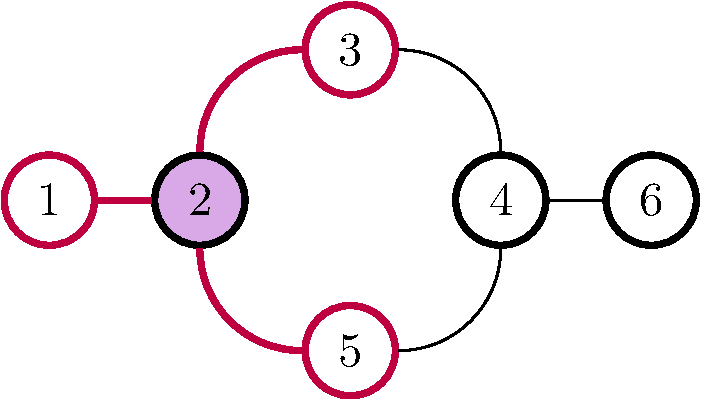
\includegraphics[width=0.8\linewidth]{Graphen/GraphNachbarschaftGrad-pdf.pdf}\\
\midrule \phantomsection \addcontentsline{toc}{section}{GraphNichtPlanarK33}\verb|Graphen/GraphNichtPlanarK33|\quad{\tiny pdf}& 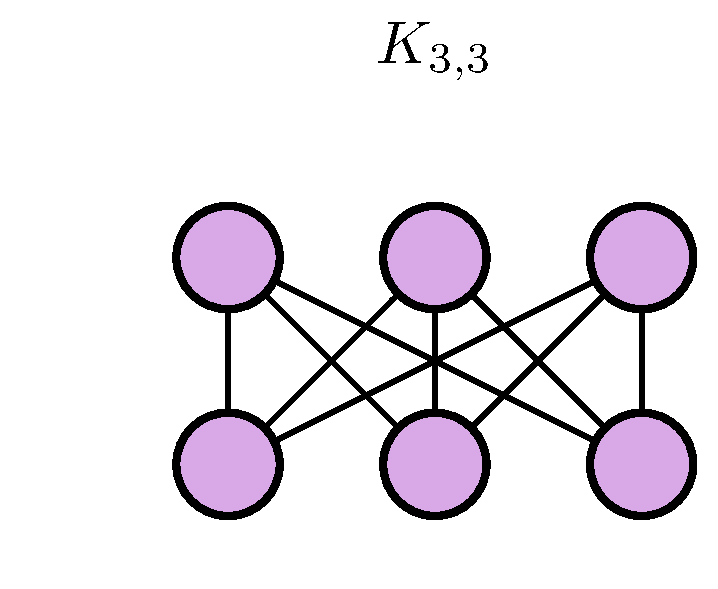
\includegraphics[width=0.8\linewidth]{Graphen/GraphNichtPlanarK33-pdf.pdf}\\
\midrule \phantomsection \addcontentsline{toc}{section}{GraphNichtPlanarK5}\verb|Graphen/GraphNichtPlanarK5|\quad{\tiny pdf}& 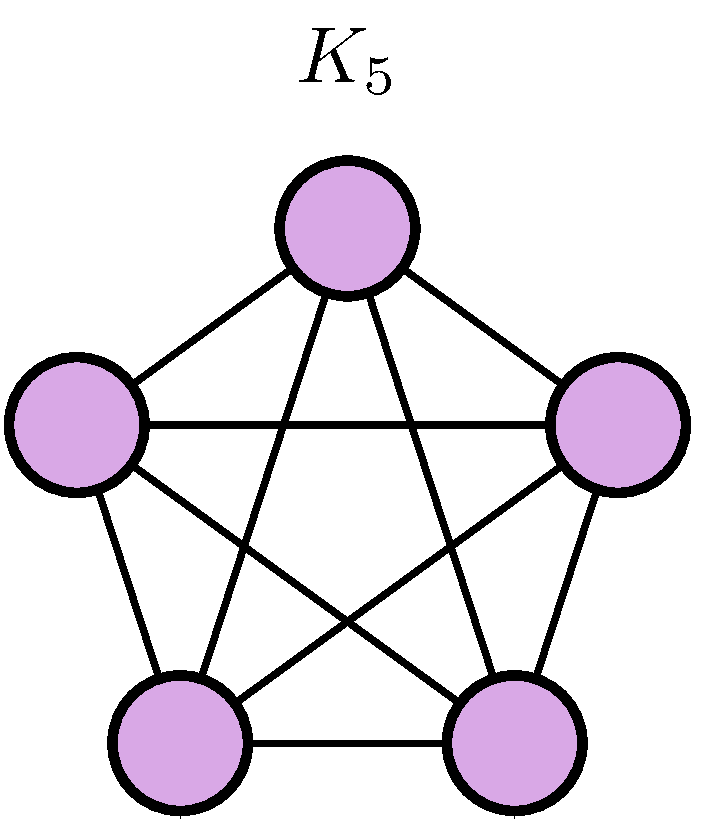
\includegraphics[width=0.8\linewidth]{Graphen/GraphNichtPlanarK5-pdf.pdf}\\
\midrule \phantomsection \addcontentsline{toc}{section}{GraphTopologie}\verb|Graphen/GraphTopologie|\quad{\tiny pdf}& 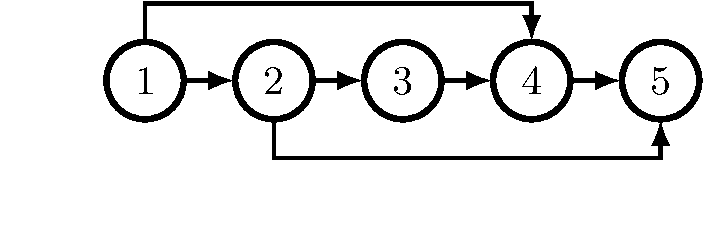
\includegraphics[width=0.8\linewidth]{Graphen/GraphTopologie-pdf.pdf}\\
\midrule \phantomsection \addcontentsline{toc}{section}{GraphWegPfad}\verb|Graphen/GraphWegPfad|\quad{\tiny pdf}& 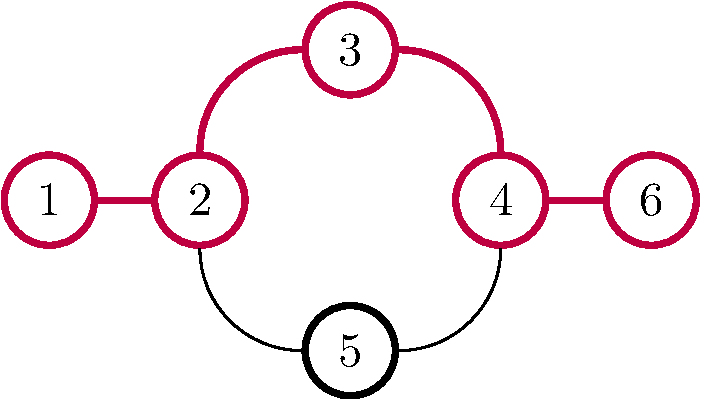
\includegraphics[width=0.8\linewidth]{Graphen/GraphWegPfad-pdf.pdf}\\
\midrule \phantomsection \addcontentsline{toc}{section}{GraphZyklus}\verb|Graphen/GraphZyklus|\quad{\tiny pdf}& 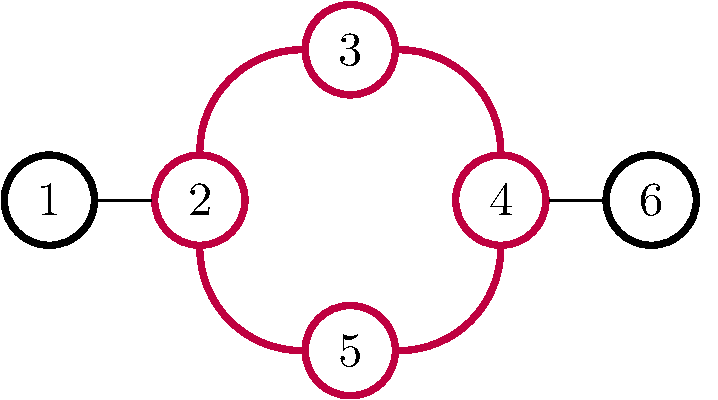
\includegraphics[width=0.8\linewidth]{Graphen/GraphZyklus-pdf.pdf}\\
\midrule 
\phantomsection \addcontentsline{toc}{chapter}{Haskell}
\phantomsection \addcontentsline{toc}{section}{HaskellTypen}\verb|Haskell/HaskellTypen|\quad{\tiny pdf}& 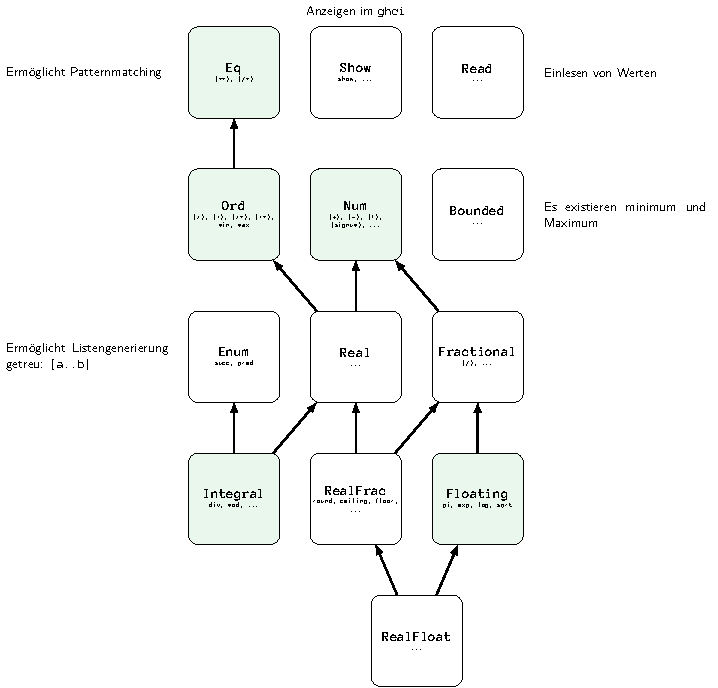
\includegraphics[width=0.8\linewidth]{Haskell/HaskellTypen-pdf.pdf}\\
\midrule \phantomsection \addcontentsline{toc}{section}{Listenoperationen}\verb|Haskell/Listenoperationen|\quad{\tiny pdf}& 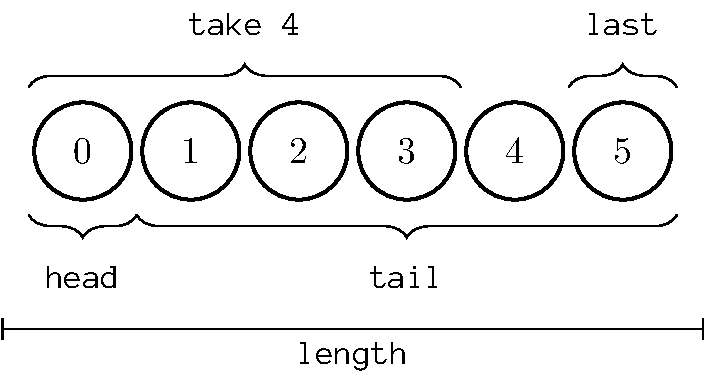
\includegraphics[width=0.8\linewidth]{Haskell/Listenoperationen-pdf.pdf}\\
\midrule 
\phantomsection \addcontentsline{toc}{chapter}{Java}
\phantomsection \addcontentsline{toc}{section}{ODBCSchematisch}\verb|Java/ODBCSchematisch|\quad{\tiny pdf}& 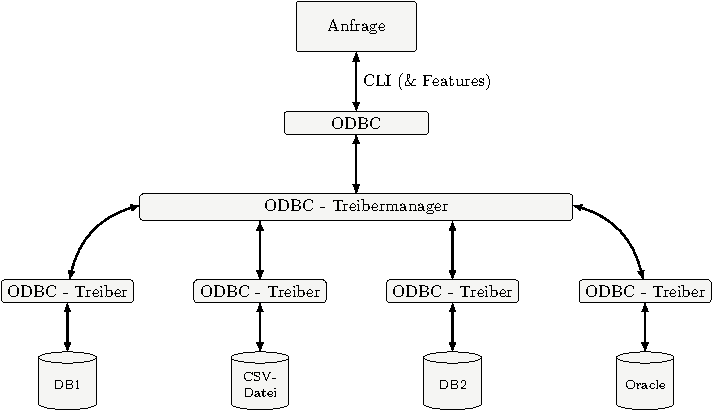
\includegraphics[width=0.8\linewidth]{Java/ODBCSchematisch-pdf.pdf}\\
\midrule \phantomsection \addcontentsline{toc}{section}{StreamDemo}\verb|Java/StreamDemo|\quad{\tiny pdf}& 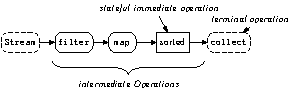
\includegraphics[width=0.8\linewidth]{Java/StreamDemo-pdf.pdf}\\
\midrule 
\phantomsection \addcontentsline{toc}{chapter}{Logik}
\phantomsection \addcontentsline{toc}{section}{KVDiagramm}\verb|Logik/KVDiagramm|\quad{\tiny pdf}& 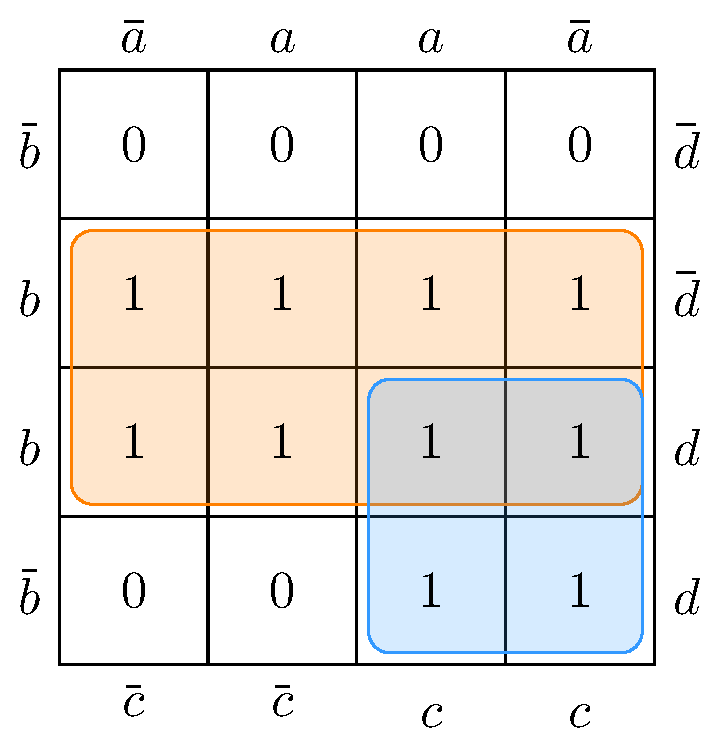
\includegraphics[width=0.8\linewidth]{Logik/KVDiagramm-pdf.pdf}\\
\midrule \phantomsection \addcontentsline{toc}{section}{KVWuerfel}\verb|Logik/KVWuerfel|\quad{\tiny pdf}& 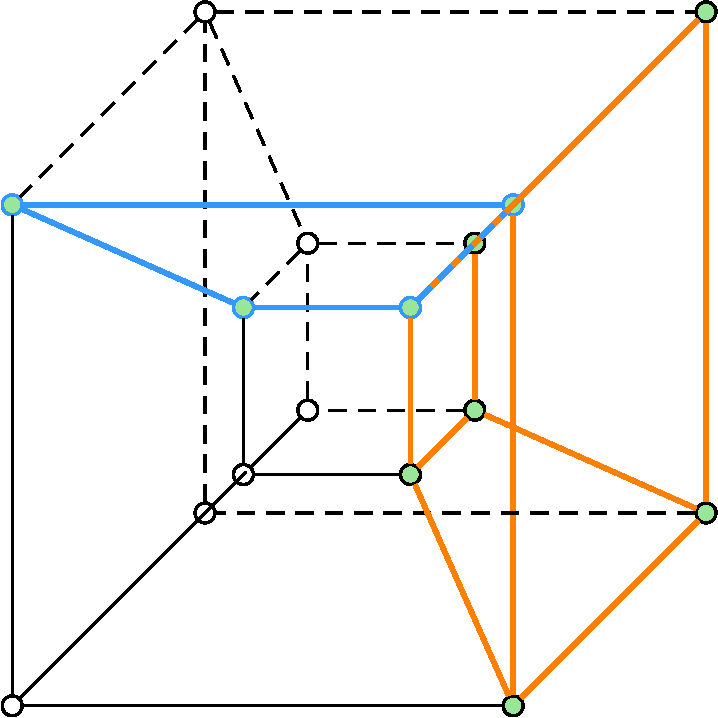
\includegraphics[width=0.8\linewidth]{Logik/KVWuerfel-pdf.pdf}\\
\midrule \phantomsection \addcontentsline{toc}{section}{QuineMCCluskeyTabelle}\verb|Logik/QuineMCCluskeyTabelle|\quad{\tiny pdf}& 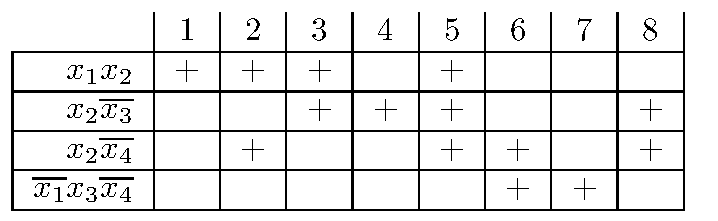
\includegraphics[width=0.8\linewidth]{Logik/QuineMCCluskeyTabelle-pdf.pdf}\\
\midrule \phantomsection \addcontentsline{toc}{section}{QuineMCCluskeyZusammenfassen}\verb|Logik/QuineMCCluskeyZusammenfassen|\quad{\tiny pdf}& 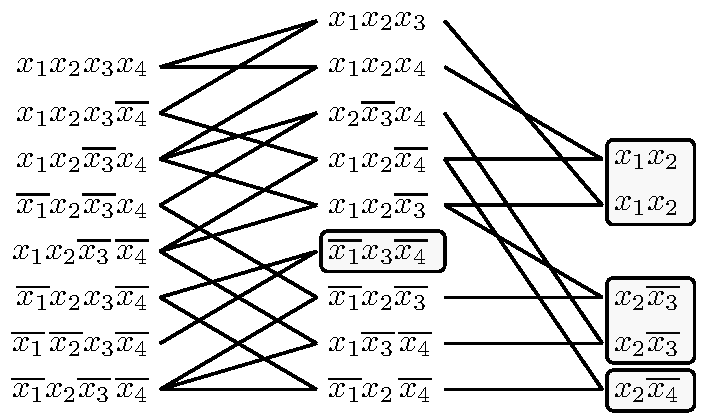
\includegraphics[width=0.8\linewidth]{Logik/QuineMCCluskeyZusammenfassen-pdf.pdf}\\
\midrule 
\phantomsection \addcontentsline{toc}{chapter}{Mengen}
\phantomsection \addcontentsline{toc}{section}{FunktionBijektiv}\verb|Mengen/FunktionBijektiv|\quad{\tiny pdf}& \includegraphics[width=0.8\linewidth]{Mengen/FunktionBijektiv-pdf.pdf}\\
\midrule \phantomsection \addcontentsline{toc}{section}{FunktionInjektiv}\verb|Mengen/FunktionInjektiv|\quad{\tiny pdf}& \includegraphics[width=0.8\linewidth]{Mengen/FunktionInjektiv-pdf.pdf}\\
\midrule \phantomsection \addcontentsline{toc}{section}{FunktionSurjektiv}\verb|Mengen/FunktionSurjektiv|\quad{\tiny pdf}& \includegraphics[width=0.8\linewidth]{Mengen/FunktionSurjektiv-pdf.pdf}\\
\midrule \phantomsection \addcontentsline{toc}{section}{Mengenmultiplikation/Mengenmultiplikation1}\verb|Mengen/Mengenmultiplikation/Mengenmultiplikation1|\quad{\tiny pdf}& \includegraphics[width=0.8\linewidth]{Mengen/Mengenmultiplikation/Mengenmultiplikation1-pdf.pdf}\\
\midrule \phantomsection \addcontentsline{toc}{section}{Mengenmultiplikation/Mengenmultiplikation2}\verb|Mengen/Mengenmultiplikation/Mengenmultiplikation2|\quad{\tiny pdf}& \includegraphics[width=0.8\linewidth]{Mengen/Mengenmultiplikation/Mengenmultiplikation2-pdf.pdf}\\
\midrule \phantomsection \addcontentsline{toc}{section}{Mengenmultiplikation/Mengenmultiplikation3}\verb|Mengen/Mengenmultiplikation/Mengenmultiplikation3|\quad{\tiny pdf}& \includegraphics[width=0.8\linewidth]{Mengen/Mengenmultiplikation/Mengenmultiplikation3-pdf.pdf}\\
\midrule \phantomsection \addcontentsline{toc}{section}{Mengenmultiplikation/Mengenmultiplikation4}\verb|Mengen/Mengenmultiplikation/Mengenmultiplikation4|\quad{\tiny pdf}& \includegraphics[width=0.8\linewidth]{Mengen/Mengenmultiplikation/Mengenmultiplikation4-pdf.pdf}\\
\midrule \phantomsection \addcontentsline{toc}{section}{VennDifferenz}\verb|Mengen/VennDifferenz|\quad{\tiny pdf}& \includegraphics[width=0.8\linewidth]{Mengen/VennDifferenz-pdf.pdf}\\
\midrule \phantomsection \addcontentsline{toc}{section}{VennSchnitt}\verb|Mengen/VennSchnitt|\quad{\tiny pdf}& \includegraphics[width=0.8\linewidth]{Mengen/VennSchnitt-pdf.pdf}\\
\midrule \phantomsection \addcontentsline{toc}{section}{VennVereinigung}\verb|Mengen/VennVereinigung|\quad{\tiny pdf}& \includegraphics[width=0.8\linewidth]{Mengen/VennVereinigung-pdf.pdf}\\
\midrule 
\phantomsection \addcontentsline{toc}{chapter}{Prozesse}
\phantomsection \addcontentsline{toc}{section}{FCFS-WorstCase}\verb|Prozesse/FCFS-WorstCase|\quad{\tiny pdf}& \includegraphics[width=0.8\linewidth]{Prozesse/FCFS-WorstCase-pdf.pdf}\\
\midrule \phantomsection \addcontentsline{toc}{section}{FCFS}\verb|Prozesse/FCFS|\quad{\tiny pdf}& \includegraphics[width=0.8\linewidth]{Prozesse/FCFS-pdf.pdf}\\
\midrule \phantomsection \addcontentsline{toc}{section}{Prozesszustaende}\verb|Prozesse/Prozesszustaende|\quad{\tiny pdf}& \includegraphics[width=0.8\linewidth]{Prozesse/Prozesszustaende-pdf.pdf}\\
\midrule 
\phantomsection \addcontentsline{toc}{chapter}{Rechner}
\phantomsection \addcontentsline{toc}{section}{ALU}\verb|Rechner/ALU|\quad{\tiny pdf}& \includegraphics[width=0.8\linewidth]{Rechner/ALU-pdf.pdf}\\
\midrule \phantomsection \addcontentsline{toc}{section}{AmpelPLA}\verb|Rechner/AmpelPLA|\quad{\tiny pdf}& \includegraphics[width=0.8\linewidth]{Rechner/AmpelPLA-pdf.pdf}\\
\midrule \phantomsection \addcontentsline{toc}{section}{BarrelShifter}\verb|Rechner/BarrelShifter|\quad{\tiny pdf}& \includegraphics[width=0.8\linewidth]{Rechner/BarrelShifter-pdf.pdf}\\
\midrule \phantomsection \addcontentsline{toc}{section}{Beispielprozessor}\verb|Rechner/Beispielprozessor|\quad{\tiny pdf}& \includegraphics[width=0.8\linewidth]{Rechner/Beispielprozessor-pdf.pdf}\\
\midrule \phantomsection \addcontentsline{toc}{section}{CLA}\verb|Rechner/CLA|\quad{\tiny pdf}& \includegraphics[width=0.8\linewidth]{Rechner/CLA-pdf.pdf}\\
\midrule \phantomsection \addcontentsline{toc}{section}{CPLD}\verb|Rechner/CPLD|\quad{\tiny pdf}& \includegraphics[width=0.8\linewidth]{Rechner/CPLD-pdf.pdf}\\
\midrule \phantomsection \addcontentsline{toc}{section}{CSA}\verb|Rechner/CSA|\quad{\tiny pdf}& \includegraphics[width=0.8\linewidth]{Rechner/CSA-pdf.pdf}\\
\midrule \phantomsection \addcontentsline{toc}{section}{DreiTorRegister}\verb|Rechner/DreiTorRegister|\quad{\tiny pdf}& \includegraphics[width=0.8\linewidth]{Rechner/DreiTorRegister-pdf.pdf}\\
\midrule \phantomsection \addcontentsline{toc}{section}{Eintorspeicher}\verb|Rechner/Eintorspeicher|\quad{\tiny pdf}& \includegraphics[width=0.8\linewidth]{Rechner/Eintorspeicher-pdf.pdf}\\
\midrule \phantomsection \addcontentsline{toc}{section}{GALPAL}\verb|Rechner/GALPAL|\quad{\tiny pdf}& \includegraphics[width=0.8\linewidth]{Rechner/GALPAL-pdf.pdf}\\
\midrule \phantomsection \addcontentsline{toc}{section}{Geraeteverwaltung}\verb|Rechner/Geraeteverwaltung|\quad{\tiny pdf}& \includegraphics[width=0.8\linewidth]{Rechner/Geraeteverwaltung-pdf.pdf}\\
\midrule \phantomsection \addcontentsline{toc}{section}{HardwareSkizze}\verb|Rechner/HardwareSkizze|\quad{\tiny pdf}& \includegraphics[width=0.8\linewidth]{Rechner/HardwareSkizze-pdf.pdf}\\
\midrule \phantomsection \addcontentsline{toc}{section}{ISA}\verb|Rechner/ISA|\quad{\tiny pdf}& \includegraphics[width=0.8\linewidth]{Rechner/ISA-pdf.pdf}\\
\midrule \phantomsection \addcontentsline{toc}{section}{LUT}\verb|Rechner/LUT|\quad{\tiny pdf}& \includegraphics[width=0.8\linewidth]{Rechner/LUT-pdf.pdf}\\
\midrule \phantomsection \addcontentsline{toc}{section}{LUTOder}\verb|Rechner/LUTOder|\quad{\tiny pdf}& \includegraphics[width=0.8\linewidth]{Rechner/LUTOder-pdf.pdf}\\
\midrule \phantomsection \addcontentsline{toc}{section}{MIPS}\verb|Rechner/MIPS|\quad{\tiny pdf}& \includegraphics[width=0.8\linewidth]{Rechner/MIPS-pdf.pdf}\\
\midrule \phantomsection \addcontentsline{toc}{section}{MuxDemuxKommunikation}\verb|Rechner/MuxDemuxKommunikation|\quad{\tiny pdf}& \includegraphics[width=0.8\linewidth]{Rechner/MuxDemuxKommunikation-pdf.pdf}\\
\midrule \phantomsection \addcontentsline{toc}{section}{MuxShannon}\verb|Rechner/MuxShannon|\quad{\tiny pdf}& \includegraphics[width=0.8\linewidth]{Rechner/MuxShannon-pdf.pdf}\\
\midrule \phantomsection \addcontentsline{toc}{section}{NAdressmaschiene}\verb|Rechner/NAdressmaschiene|\quad{\tiny pdf}& \includegraphics[width=0.8\linewidth]{Rechner/NAdressmaschiene-pdf.pdf}\\
\midrule \phantomsection \addcontentsline{toc}{section}{PLA}\verb|Rechner/PLA|\quad{\tiny pdf}& \includegraphics[width=0.8\linewidth]{Rechner/PLA-pdf.pdf}\\
\midrule \phantomsection \addcontentsline{toc}{section}{PLAAmpel}\verb|Rechner/PLAAmpel|\quad{\tiny pdf}& \includegraphics[width=0.8\linewidth]{Rechner/PLAAmpel-pdf.pdf}\\
\midrule \phantomsection \addcontentsline{toc}{section}{PROM}\verb|Rechner/PROM|\quad{\tiny pdf}& \includegraphics[width=0.8\linewidth]{Rechner/PROM-pdf.pdf}\\
\midrule \phantomsection \addcontentsline{toc}{section}{Pages}\verb|Rechner/Pages|\quad{\tiny pdf}& \includegraphics[width=0.8\linewidth]{Rechner/Pages-pdf.pdf}\\
\midrule \phantomsection \addcontentsline{toc}{section}{Physik/DiodenStromstaerke}\verb|Rechner/Physik/DiodenStromstaerke|\quad{\tiny pdf}& \includegraphics[width=0.8\linewidth]{Rechner/Physik/DiodenStromstaerke-pdf.pdf}\\
\midrule \phantomsection \addcontentsline{toc}{section}{Physik/Metastabil}\verb|Rechner/Physik/Metastabil|\quad{\tiny pdf}& \includegraphics[width=0.8\linewidth]{Rechner/Physik/Metastabil-pdf.pdf}\\
\midrule \phantomsection \addcontentsline{toc}{section}{Physik/TransistorStoertoleranz}\verb|Rechner/Physik/TransistorStoertoleranz|\quad{\tiny pdf}& \includegraphics[width=0.8\linewidth]{Rechner/Physik/TransistorStoertoleranz-pdf.pdf}\\
\midrule \phantomsection \addcontentsline{toc}{section}{RegisterParallel}\verb|Rechner/RegisterParallel|\quad{\tiny pdf}& \includegraphics[width=0.8\linewidth]{Rechner/RegisterParallel-pdf.pdf}\\
\midrule \phantomsection \addcontentsline{toc}{section}{RegisterSeriell}\verb|Rechner/RegisterSeriell|\quad{\tiny pdf}& \includegraphics[width=0.8\linewidth]{Rechner/RegisterSeriell-pdf.pdf}\\
\midrule \phantomsection \addcontentsline{toc}{section}{Shiftregister}\verb|Rechner/Shiftregister|\quad{\tiny pdf}& \includegraphics[width=0.8\linewidth]{Rechner/Shiftregister-pdf.pdf}\\
\midrule \phantomsection \addcontentsline{toc}{section}{Speicherhierarchie}\verb|Rechner/Speicherhierarchie|\quad{\tiny pdf}& \includegraphics[width=0.8\linewidth]{Rechner/Speicherhierarchie-pdf.pdf}\\
\midrule \phantomsection \addcontentsline{toc}{section}{StackExample}\verb|Rechner/StackExample|\quad{\tiny pdf}& \includegraphics[width=0.8\linewidth]{Rechner/StackExample-pdf.pdf}\\
\midrule \phantomsection \addcontentsline{toc}{section}{Stackmaschiene}\verb|Rechner/Stackmaschiene|\quad{\tiny pdf}& \includegraphics[width=0.8\linewidth]{Rechner/Stackmaschiene-pdf.pdf}\\
\midrule \phantomsection \addcontentsline{toc}{section}{StackmaschieneSimpler}\verb|Rechner/StackmaschieneSimpler|\quad{\tiny pdf}& \includegraphics[width=0.8\linewidth]{Rechner/StackmaschieneSimpler-pdf.pdf}\\
\midrule 
\phantomsection \addcontentsline{toc}{chapter}{Schaltkreis}
\phantomsection \addcontentsline{toc}{section}{Addier-Subtrahierer}\verb|Schaltkreis/Addier-Subtrahierer|\quad{\tiny pdf}& \includegraphics[width=0.8\linewidth]{Schaltkreis/Addier-Subtrahierer-pdf.pdf}\\
\midrule \phantomsection \addcontentsline{toc}{section}{Demultiplexer}\verb|Schaltkreis/Demultiplexer|\quad{\tiny pdf}& \includegraphics[width=0.8\linewidth]{Schaltkreis/Demultiplexer-pdf.pdf}\\
\midrule \phantomsection \addcontentsline{toc}{section}{KomplexerSchaltkreis}\verb|Schaltkreis/KomplexerSchaltkreis|\quad{\tiny pdf}& \includegraphics[width=0.8\linewidth]{Schaltkreis/KomplexerSchaltkreis-pdf.pdf}\\
\midrule \phantomsection \addcontentsline{toc}{section}{SynchronzaehlerDFF}\verb|Schaltkreis/SynchronzaehlerDFF|\quad{\tiny pdf}& \includegraphics[width=0.8\linewidth]{Schaltkreis/SynchronzaehlerDFF-pdf.pdf}\\
\midrule \phantomsection \addcontentsline{toc}{section}{SynchronzaehlerTFF}\verb|Schaltkreis/SynchronzaehlerTFF|\quad{\tiny pdf}& \includegraphics[width=0.8\linewidth]{Schaltkreis/SynchronzaehlerTFF-pdf.pdf}\\
\midrule \phantomsection \addcontentsline{toc}{section}{Volladdierer}\verb|Schaltkreis/Volladdierer|\quad{\tiny pdf}& \includegraphics[width=0.8\linewidth]{Schaltkreis/Volladdierer-pdf.pdf}\\
\midrule 
\phantomsection \addcontentsline{toc}{chapter}{Software}
\phantomsection \addcontentsline{toc}{section}{DreiSchichtenArchitektur}\verb|Software/DreiSchichtenArchitektur|\quad{\tiny pdf}& \includegraphics[width=0.8\linewidth]{Software/DreiSchichtenArchitektur-pdf.pdf}\\
\midrule \phantomsection \addcontentsline{toc}{section}{Meta/ProgrammierparadigmenUeberblick}\verb|Software/Meta/ProgrammierparadigmenUeberblick|\quad{\tiny pdf}& \includegraphics[width=0.8\linewidth]{Software/Meta/ProgrammierparadigmenUeberblick-pdf.pdf}\\
\midrule \phantomsection \addcontentsline{toc}{section}{ModelViewController}\verb|Software/ModelViewController|\quad{\tiny pdf}& \includegraphics[width=0.8\linewidth]{Software/ModelViewController-pdf.pdf}\\
\midrule \phantomsection \addcontentsline{toc}{section}{RegexExample}\verb|Software/RegexExample|\quad{\tiny pdf}& \includegraphics[width=0.8\linewidth]{Software/RegexExample-pdf.pdf}\\
\midrule \phantomsection \addcontentsline{toc}{section}{SQL/SQLFields}\verb|Software/SQL/SQLFields|\quad{\tiny pdf}& \includegraphics[width=0.8\linewidth]{Software/SQL/SQLFields-pdf.pdf}\\
\midrule \phantomsection \addcontentsline{toc}{section}{SQL/SQLFieldsDCL}\verb|Software/SQL/SQLFieldsDCL|\quad{\tiny pdf}& \includegraphics[width=0.8\linewidth]{Software/SQL/SQLFieldsDCL-pdf.pdf}\\
\midrule \phantomsection \addcontentsline{toc}{section}{SQL/SQLFieldsDDL}\verb|Software/SQL/SQLFieldsDDL|\quad{\tiny pdf}& \includegraphics[width=0.8\linewidth]{Software/SQL/SQLFieldsDDL-pdf.pdf}\\
\midrule \phantomsection \addcontentsline{toc}{section}{SQL/SQLFieldsDML}\verb|Software/SQL/SQLFieldsDML|\quad{\tiny pdf}& \includegraphics[width=0.8\linewidth]{Software/SQL/SQLFieldsDML-pdf.pdf}\\
\midrule \phantomsection \addcontentsline{toc}{section}{SQL/SQLFieldsDQL}\verb|Software/SQL/SQLFieldsDQL|\quad{\tiny pdf}& \includegraphics[width=0.8\linewidth]{Software/SQL/SQLFieldsDQL-pdf.pdf}\\
\midrule \phantomsection \addcontentsline{toc}{section}{ThreadStates}\verb|Software/ThreadStates|\quad{\tiny pdf}& \includegraphics[width=0.8\linewidth]{Software/ThreadStates-pdf.pdf}\\
\midrule \phantomsection \addcontentsline{toc}{section}{UML/UMLCompositePattern}\verb|Software/UML/UMLCompositePattern|\quad{\tiny pdf}& \includegraphics[width=0.8\linewidth]{Software/UML/UMLCompositePattern-pdf.pdf}\\
\midrule \phantomsection \addcontentsline{toc}{section}{UML/UMLDecoratorPattern}\verb|Software/UML/UMLDecoratorPattern|\quad{\tiny pdf}& \includegraphics[width=0.8\linewidth]{Software/UML/UMLDecoratorPattern-pdf.pdf}\\
\midrule \phantomsection \addcontentsline{toc}{section}{UML/UMLExample}\verb|Software/UML/UMLExample|\quad{\tiny pdf}& \includegraphics[width=0.8\linewidth]{Software/UML/UMLExample-pdf.pdf}\\
\midrule \phantomsection \addcontentsline{toc}{section}{UML/UMLFactoryPattern}\verb|Software/UML/UMLFactoryPattern|\quad{\tiny pdf}& \includegraphics[width=0.8\linewidth]{Software/UML/UMLFactoryPattern-pdf.pdf}\\
\midrule \phantomsection \addcontentsline{toc}{section}{UML/UMLObserverPattern}\verb|Software/UML/UMLObserverPattern|\quad{\tiny pdf}& \includegraphics[width=0.8\linewidth]{Software/UML/UMLObserverPattern-pdf.pdf}\\
\midrule \phantomsection \addcontentsline{toc}{section}{UML/UMLSEQObserverPattern}\verb|Software/UML/UMLSEQObserverPattern|\quad{\tiny pdf}& \includegraphics[width=0.8\linewidth]{Software/UML/UMLSEQObserverPattern-pdf.pdf}\\
\midrule \phantomsection \addcontentsline{toc}{section}{UML/UMLSEQObserverPatternAdapted}\verb|Software/UML/UMLSEQObserverPatternAdapted|\quad{\tiny pdf}& \includegraphics[width=0.8\linewidth]{Software/UML/UMLSEQObserverPatternAdapted-pdf.pdf}\\
\midrule \phantomsection \addcontentsline{toc}{section}{UML/UMLStateDiagramExample}\verb|Software/UML/UMLStateDiagramExample|\quad{\tiny pdf}& \includegraphics[width=0.8\linewidth]{Software/UML/UMLStateDiagramExample-pdf.pdf}\\
\midrule \phantomsection \addcontentsline{toc}{section}{UML/UMLThread}\verb|Software/UML/UMLThread|\quad{\tiny pdf}& \includegraphics[width=0.8\linewidth]{Software/UML/UMLThread-pdf.pdf}\\
\midrule \phantomsection \addcontentsline{toc}{section}{XML/XMLUebersicht}\verb|Software/XML/XMLUebersicht|\quad{\tiny pdf}& \includegraphics[width=0.8\linewidth]{Software/XML/XMLUebersicht-pdf.pdf}\\
\midrule 
\phantomsection \addcontentsline{toc}{chapter}{Sprachen}
\phantomsection \addcontentsline{toc}{section}{CYKAlgorithmus}\verb|Sprachen/CYKAlgorithmus|\quad{\tiny pdf}& \includegraphics[width=0.8\linewidth]{Sprachen/CYKAlgorithmus-pdf.pdf}\\
\midrule \phantomsection \addcontentsline{toc}{section}{ChomskyHierarchie}\verb|Sprachen/ChomskyHierarchie|\quad{\tiny pdf}& \includegraphics[width=0.8\linewidth]{Sprachen/ChomskyHierarchie-pdf.pdf}\\
\midrule \phantomsection \addcontentsline{toc}{section}{Grammatik}\verb|Sprachen/Grammatik|\quad{\tiny pdf}& \includegraphics[width=0.8\linewidth]{Sprachen/Grammatik-pdf.pdf}\\
\midrule \bottomrule
\end{tabularx}
\end{document}